\chapter{Methodology}
\label{sec:Method}
\label{Chapter3} % For referencing the chapter elsewhere, use \ref{Chapter3}

% Introduce the purpose of this chapter.
% Reiterate your research aim: enhancing static malware analysis with LLMs and RAG.
% Provide a brief overview of the methodology, including data sources,
% architecture, evaluation strategy, and toolchain.
TODO...

\section{Research Design}
% Describe the nature of your research: exploratory, experimental, comparative.
% Explain the reasoning for using a prototype-based implementation and evaluation.
% Emphasize that your approach avoids LLM fine-tuning and instead relies on
% prompt engineering and external context via RAG.
TODO...

\section{System Architecture}
% Provide a high-level description of your system pipeline.
% Include a diagram (later) showing flow: malware sample → static feature extraction → retrieval → prompt generation → LLM response.
% List major system components and their interactions.

This section outlines the overview of the pipeline architecture. These steps have been designed to
modularize the analysis, ensure reproducibility and allow for algorithmic changes whenever needed.
Below, the diagram of the pipeline elements is displayed along with an overview on each of them.

\begin{figure}[htbp]
    \centering
    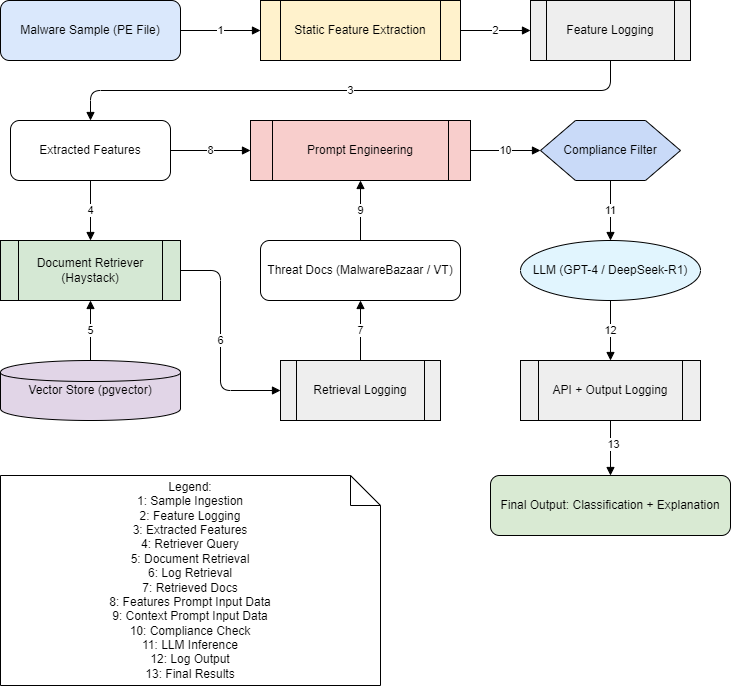
\includegraphics[width=0.85\textwidth]{pipeline-diagram.png}
    \caption{System Pipeline Diagram}
    \label{fig:pipeline_diagram}
\end{figure}

\FloatBarrier

\begin{enumerate}
    \item \textbf{Malware Sample Ingestion:} Raw malware binaries (e.g., PE files) are sourced from public repositories such as MalwareBazaar or accessed via API from VirusTotal. Each file is stored with a unique identifier (e.g., SHA256 hash).

    \item \textbf{Static Feature Extraction:} Using tools such as \texttt{pefile}, the system extracts static attributes from the malware, including:
          \begin{itemize}
              \item PE header metadata
              \item Imported API calls
              \item Section structure and entropy
              \item Printable strings
          \end{itemize}

    \item \textbf{Log Feature Extraction:} All extracted features are logged with timestamps, sample identifiers, and summary statistics.

    \item \textbf{Feature-Based Retrieval Query:} The extracted static features are embedded into vector representations (if needed) and used as queries to a semantic search index.

    \item \textbf{Document Retrieval:} Relevant documents (e.g., threat reports,
          malware family descriptions) are retrieved from an external datastore to be
          provided as context.

    \item \textbf{Log Retrieval Step:} Retrieval activity is logged, including query terms, matching document IDs, retrieval time, and the data source used (e.g., VirusTotal vs. local data).

    \item \textbf{Prompt Construction:} Retrieved documents and extracted features are formatted into structured prompts. Templates are used to ensure consistent formatting across LLM queries.

    \item \textbf{Compliance Check Module:} Before sending prompts to the LLM, a filtering mechanism ensures that no disallowed content (e.g., malware payloads, sensitive data, proprietary code) is included.

    \item \textbf{LLM Inference (GPT-4 / DeepSeek-R1):} The prompt is passed to a large language model (either GPT-4 or DeepSeek-R1) to generate:
          \begin{itemize}
              \item Malware family classification
              \item Explanation or justification of the classification
              \item Comparative analysis against known malware types
          \end{itemize}

    \item \textbf{Log API Call:} Each API interaction is logged, including:
          \begin{itemize}
              \item Model version and endpoint
              \item Prompt metadata (not full text for privacy)
              \item Token usage, latency, and return timestamp
          \end{itemize}

    \item \textbf{Output Generation:} The model output (classification + explanation) is presented to the user or stored for evaluation.

    \item \textbf{Results Logging and Storage:} Final outputs, along with model metadata and hash references, are stored for downstream analysis or human review.
\end{enumerate}

\section{Data Sources}
% Describe where you obtain your malware samples and intelligence documents.
% Malware sources:
%   - MalwareBazaar for static binaries and metadata.
%   - VirusTotal (optional, via API) for reports and behavior data.
%     Detail any preprocessing steps: parsing PE headers, extracting bytecode,
%     API call strings, etc.
TODO...

\section{Retrieval-Augmented Generation (RAG) Pipeline}
% Explain how RAG is constructed using Haystack and pgvector.
% Describe:
%   - Embedding model used to vectorize documents.
%   - How documents (e.g., malware reports) are stored in PostgreSQL.
%   - How semantic retrieval is performed and injected into the LLM prompt.
%     Clarify how this improves contextual relevance and grounding in known
%     threat data.
TODO...

\section{Prompt Engineering}
% Discuss how you craft prompts for different tasks: classification, explanation, and comparison.
% Include examples of how static features and retrieved context are structured in the prompt.
% Explain the decision to use GPT-4 and/or DeepSeek-R1 in inference-only mode.
TODO...

\section{Toolchain}
This section outlines the used tooling for the experiments and some discussion on why they were
chosen.

\subsection{Programming Language and Environment}
% Python is used for implementation.
% PDM (Python Development Master) manages dependencies and virtual environments.
TODO...

\subsection{Language Models}
% GPT-4 (via OpenAI API) and/or DeepSeek-R1 are used for inference.
% Models are not fine-tuned; they rely on prompt engineering and external
% retrieval for task performance.
TODO...

\subsection{RAG Framework and Storage}
% Haystack is used to build the retrieval pipeline.
% PostgreSQL with pgvector is used to store and query vector embeddings of
% malware-related documents.
TODO...

\subsection{Malware Intelligence Sources}
% MalwareBazaar is used to obtain real-world malware samples and metadata.
% VirusTotal may be used (via API) to enrich data with threat reports and
% behavioral indicators.
TODO...

\subsection{Evaluation and Visualization}
% Scikit-learn is used to compute performance metrics (e.g., accuracy, F1 score).
% Pandas and Matplotlib are used for data handling and visualization.
% All experiments are version-controlled and reproducible via PDM.
TODO...

\section{Evaluation Framework}
% Define your evaluation metrics: accuracy, efficiency, interpretability.
% Describe baseline comparisons against traditional static malware classifiers (if applicable).
% Discuss any human-in-the-loop components for evaluating explanation quality.
TODO...

\section{Reliability, Validity, and Limitations}
% Discuss how reproducibility is ensured via version control, fixed seeds, and public datasets.
% Address limitations:
%   - Limited to static analysis.
%   - Dependent on retrieval quality and LLM reliability.
%   - No user-study or adversarial robustness testing (unless planned).
TODO...

\section{Ethical Considerations}
% Ensure ethical use of malware datasets.
% Describe safety protocols: no execution of live malware, all samples are statically analyzed.
% Highlight responsible use of LLMs and privacy-conscious data handling if using
% VirusTotal.
TODO...

\section{Summary}
% Recap the methodology structure and justify how it addresses your research questions.
% Set up the transition into the next chapter, where implementation details or
% results will follow.
TODO...
